\documentclass[onecolumn, crcready]{iosart2c}
\usepackage{graphicx}
\usepackage[ampersand]{easylist}
\usepackage{amssymb}
\usepackage{lscape}
\usepackage{multirow}
\usepackage{longtable}
\usepackage{tikz}
\usepackage{array}
\usepackage{booktabs}
\usepackage{rotating}
\usepackage{listings}
\usepackage{pifont}
\def\checkmark{\tikz\fill[scale=0.4](0,.35) -- (.25,0) -- (1,.7) -- (.25,.15) -- cycle;}

\graphicspath{ {figures/} }
\newcolumntype{L}{>{\arraybackslash}m{13cm}}

\begin{document}
\begin{frontmatter}


\title{An Objective Assessment Framework \& Tool for Linked Data Quality}
\subtitle{Enriching Dataset Profiles with Quality Indicators}
\author[A,B]{Ahmad Assaf}, \author[A]{Aline Senart} and
\author[B]{Rapha\"{e}l Troncy}
\address[A]{SAP Research, SAP Labs France SAS,\\
805 avenue du Dr. Maurice Donat, BP 1216, 06254 Mougins Cedex, France\\
\email{first.last@sap.com}}
\address[B]{EURECOM,\\
2229 route des cretes, 06560 Sophia Antipolis, France\\
\email{first.last@eurecom.fr}}


\begin{abstract}
The standardization of Semantic Web technologies and specifications has resulted in a staggering volume of data being published. The Linked Open Data (LOD) is a gold mine for organizations trying to leverage external data sources in order to produce more informed business decisions. However, the heterogeneous nature of data sources reflects directly on the data quality as these sources often contain inconsistent as well as misinterpreted and incomplete information. Traditional data quality is a thoroughly researched field with several benchmarks and frameworks to grasp its dimensions. Ensuring data quality in Linked Open Data is much more complex. It consists of structured information supported by models, ontologies and vocabularies and contains queryable endpoints and links. In this paper, we first propose an objective assessment framework for Linked Data quality. In a previous work, we identified potential quality issues of Linked Data and listed quality principles for all stages of data management. In this paper, we build upon this work but focus only on the objective quality indicators based on metrics that can be automatically measured. Secondly, we surveyed the landscape of Linked Data quality tools to discover that they only cover a subset of the proposed quality indicators. As a result, we present an extensible quality measurement tool that helps on one hand data owners to rate the quality of their datasets and get some hints on possible improvements, and on the other hand data consumers to choose their data sources from a ranked set. We evaluate this tool by measuring the quality of the LOD cloud. The results demonstrate that the general state of the datasets needs attention as they mostly have low completeness, provenance, licensing and comprehensibility quality scores.
\end{abstract}

\begin{keyword}
Data Quality\sep Linked Data\sep Quality Framework\sep Semantic Web\sep Objective Quality
\end{keyword}
\end{frontmatter}

\section{Introduction}
In the last few years the Semantic Web gained a momentum supported by the introduction of many related initiatives like the Linked Open Data (LOD)\footnote{http://lod-cloud.net}. From 12 datasets cataloged in 2007, the Linked Open Data cloud has grown to nearly 1000 datasets containing more than 82 billion triples. Data is being published by both public and private sectors and covers a diverse set of domains from life sciences to military. This success lies in the cooperation between data publishers and consumers where users are empowered to find, share and combine information in their applications easily.

We are entering an era where open is the new default. Governments, universities, organizations and even individuals are publicly publishing huge amounts of open data. This openness should be accompanied with a certain level of trust or guarantees about the quality of data. The Linked Open Data is a gold mine for those trying to leverage external data sources in order to produce more informed business decisions \cite{Boyd2011}. However, the heterogeneous nature of sources reflects directly on the data quality as these sources often contain inconsistent as well as misinterpreted and incomplete information.

Traditional data quality is a thoroughly researched field with several benchmarks and frameworks to grasp its dimensions \cite{Kahn2002}\cite{Stvilia2007}\cite{Wang1996}. Data quality principles typically rely on many subjective indicators that are complex to measure automatically. The quality of data in indeed realized when it is used \cite{juran-j-1999-quality}, thus directly relating to the ability of satisfying users' continuous needs.

Web documents that are by nature unstructured and interlinked require different quality metrics and assessment techniques than traditional datasets. For example, the importance and quality of Web documents can be subjectively calculated via algorithms like Page Rank \cite{ Lawrence981}.
Ensuring data quality in Linked Open Data is much more complex. It consists of structured information supported by models, ontologies and vocabularies and contains queryable endpoints and links. This makes data quality assurance a challenge. Despite the fact that Linked Open Data quality is a trending and highly demanded topic, very few efforts are currently trying to standardize, track and formalize frameworks to issue scores or certificates that will help data consumers in their integration tasks.\\

Data quality assessment is the process of evaluating if a piece of data meets the consumers need in a specific use case \cite{Bizer:2009:QIF:1482178.1482280}. The dimensionality of data quality makes it dependent on the task and users requirements. For example, DBpedia \cite{bizer_dbpedia_2009} is a knowledge base containing data extracted from structured and semi-structured sources. It is used in a variety of applications  e.g. annotation systems \cite{Mendes:2011:DSS:2063518.2063519}, exploratory search \cite{Marie:2013:DHO:2506182.2506185} and recommendation engines \cite{conf/iir/MirizziNROS12}. However, DBpedia's data isn't integrated into critical systems e.g. life critical (medical applications) or safety critical (aviation applications) as its data quality is found to be insufficient. In this paper, we first propose a comprehensive objective framework to evaluate the quality of Linked Data sources. Secondly, we present an extensible quality measurement tool that helps on one hand data owners to rate the quality of their dataset and get some hints on possible improvements, and on the other hand data consumers to choose their data sources from a ranked set. The aim of this paper is to provide researchers and practitioners with a comprehensive understanding of the objective issues surrounding Linked Data quality.\\

The framework we propose is based on a refinement of the data quality principles proposed in our previous work \cite{assaf2012} and those surveyed in \cite{Framework2012}. Some attributes have been grouped for more detailed quality assessments while we have also extended them by adding for each attribute a set of objective indicators. These indicators are measures that provide users with quality metrics measurable by tools regardless of the use case. For example, when measuring the quality of DBpedia dataset, an objective metric would be the availability of human or machine readable license information rather than the trustworthiness of the publishers.

Furthermore, we surveyed the landscape of Linked Data quality tools to discover that they only cover a subset of the proposed objective quality indicators. As a result, we extend Roomba\footnote{https://github.com/ahmadassaf/opendata-checker} which is a framework to assess and build dataset profiles with an extensible quality measurement tool and evaluate it by measuring the quality of the LOD cloud group. The results demonstrate that the general quality of LOD cloud needs more attention as most of the datasets suffer from various quality issues.\\

This paper is structured as follows: Section 2 presents the various data quality assessment methodologies, Section 3 presents our framework with its objective quality measures and indicators; Section 4 presents our tool for evaluating those indicators; Section 5 presents our evaluation and experiments running this tool on the LOD cloud group; Section 6 reviews the existing tools and frameworks in the Linked Open Data quality landscape; Section 7 presents concluding remarks and identifies future work.

\section{Data Quality Assessment}

In \cite{Framework2012}, the authors present a comprehensive systematic review of data quality assessment methodologies applied to LOD. They have extracted 26 quality dimensions and a total of 110 objective and subjective quality indicators. However, some of those objective indicators are dependent on the use case thus there is no clear separation on what can be automatically measured. For example, data completeness is generally a subjective dimension. However, the authors specified that the detection of the degree on which all the real-world objects are represented, detection of number of missing values for specific property and detection of the degree to which instances in the dataset are interlinked are considered as objective indicators given the presence of a gold standard or the original data source to compare with. Moreover, lots of the defined performance dimensions like low latency, high throughput or scalability of a data source were defined as objective but are still dependent on multiple subjective factors like network congestion. In addition, there were some missing objective indicators vital to the quality of LOD e.g. indication of the openness of the dataset.\\

The ODI certificate\footnote {https://certificates.theodi.org/} provides a description of the published data quality in plain English. It aspires to act as a mark of approval that helps publishers understand how to publish good open data and users how to use it. It gives publishers the ability to provide assurance and support on their data while encouraging further improvements through an ascending scale.

ODI comes as an online and free questionnaire for data publishers focusing on certain characteristics about their data. The questions are classified into the following categories: general information (about dataset, publisher and type of release), legal information (e.g., rights to publish), licensing, privacy (e.g., whether individuals can be identified), practical information (e.g., how to reach the data), quality, reliability, technical information (e.g., format and type of data) and social information (e.g., contacts, communities, etc.). Based on the information provided  by the data  publisher,  a certificate  is created  with one of four different ratings.\\
Although ODI is a great initiative, the issued certificates are “self-certified“. ODI does not verify or review submissions but retains the right to revoke a certificate at any time. The dynamicity of Linked Data  makes it also very difficult to update the certificates manually, especially when these changes are frequent and affect multiple categories. There is clearly a need for automatic certification which can be supplemented with some manual input for categories that cannot be processed by machines.\\

The emerging critical need for large, distributed, heterogeneous, and complex structured datasets identified the necessity to establish industry cooperation between vendors of RDF and Graph database technologies in developing, endorsing, and publishing reliable and insightful benchmark results. The Linked Data Benchmark Council (LDBC)\footnote{http://ldbc.eu/} aims to bridge the gap between the industry and the new trending stack of semantic technologies and their vendors. \\ LDBC more specifically aims at developing new benchmarks that will lead to significant progress in scalability, storage, indexing and query optimization techniques to become the de facto standard for publishing performance results. LDBC is a promising initiative, but it is still work in progress with the final report expected on the first quarter of 2015.\\

In \cite{DBLP:conf/i-semantics/RulaZ14}, the authors propose a methodology for assessing Linked Data quality. It consists of three main steps: (1) requirement analysis, (2) quality assessment and (3) quality improvement. Considering the multidimensionality of data quality, the methodology requires users to provide the details of a use case or a scenario that describes the intended usage of the data. Moreover, quality issues identification is done with the help of a checklist. The user must have prior knowledge about the details of the data in order to fill this list.
Tools implementing the proposed methodology should be able to generate comprehensive quality measures. However, they will require heavy manual intervention and deep knowledge on the data examined. These issues highly affect detecting quality issue on large scale.\\

Despite all the recent efforts in providing frameworks and tools for data quality in Linked Open Data, there is still no automatic framework for the objective assessment of Linked Data quality.

\section{Objective Linked Data Quality Classification}
% Shorten this %
In this section, we present the objective Linked Data quality framework based on the refinement of our previous work \cite{assaf2012} and those surveyed in \cite{Framework2012}.\\

The basic idea behind Linked Data is that its usefulness increases when it is more interlinked with other datasets. Tim Berners-Lee defined four main principles for publishing data that can ensure a certain level of uniformity reflecting directly data's usability \cite{tim:linkedata}:\\

\begin{easylist}[itemize]
\ListProperties( Hang=true, Progressive=3ex, Style*=\tiny$\blacksquare$  )
& {\bf Make the data available on the Web}: assign URIs to identify things.
& {\bf Make the data machine readable}: use HTTP URIs so that looking up these names is easy.
& {\bf Use publishing standards}: when the lookup is done provide useful information using standards like RDF.
& {\bf Link your data}: include links to other resources to enable users to discover more things.\\
\end{easylist}

\noindent
Building on these principles, we group the quality attributes into four main categories:\\
\begin{easylist}[itemize]
\ListProperties( Hang=true, Progressive=3ex, Style*=\tiny$\blacksquare$  )
& {\bf Quality of the entities }: quality indicators that focus on the data at the instance level.
& {\bf Quality of the dataset}: quality indicators at the dataset level.
& {\bf Quality of the semantic model}: quality indicators that focus on the semantic models, vocabularies and ontologies.
& {\bf Quality of the linking process}: quality indicators that focus on the inbound and outbound links between datasets.\\
\end{easylist}

In our previous work \cite{assaf2012} we have identified 24 different Linked Data quality attributes. In this paper, we refine these attributes into a condensed framework of 10 objective measures. Since these measures are rather abstract, we should rely on quality indicators that reflect data quality \cite{flemming2010}. In this paper, we transform the quality indicators presented as a set of questions in \cite{assaf2012} into more concrete quality indicator metrics.\\
Independent indicators for entity quality are mainly subjective e.g. the degree to which all the real-world objects are represented, the scope and level of details, etc. However, since entities are governed by the underlying model, we have grouped their indicators with those of the modeling quality. Table 1 lists the refined measures alongside their quality indicators. These attributes are presented in the following sections. \\

\begin{center}
{\footnotesize
\begin{longtable}[h]{|c|c|c|l|}
\caption[Objective Linked Data Quality Framework]{Objective Linked Data Quality Framework} \label{DQM} \\

\hline \multicolumn{1}{|c|}{\textbf{Quality Attribute}} & \multicolumn{1}{c|}{\textbf{Quality Category}} & \multicolumn{1}{c|}{\textbf{ID}} & \multicolumn{1}{c|}{\textbf{Quality Indicator}} \\ \hline
\endfirsthead

\multicolumn{4}{c}%
{{\bfseries \tablename\ \thetable{} Objective Linked Data Quality Framework}} \\
\hline \multicolumn{1}{|c|}{\textbf{Quality Attribute}} &
\multicolumn{1}{c|}{\textbf{Quality Category}} & \textbf{ID} &
\multicolumn{1}{c|}{\textbf{Quality Indicator}} \\ \hline
\endhead

\multicolumn{4}{|r|}{{Continued on next page}} \\ \hline
\endfoot

\endlastfoot

\multirow{15}{*}{Completeness}
 & \multirow{5}{*}{Dataset Level} & 1 & Existence of supporting structured metadata  \cite{Hogan2010}\tabularnewline
\cline{3-4}
 &  & 2 & Supports multiple serializations \cite{Framework2012}\tabularnewline
\cline{3-4}
 &  & 3 & Has different data access points \tabularnewline
\cline{3-4}
 &  & 4 & Uses datasets description vocabularies \tabularnewline
\cline{3-4}
 &  & 5 & Existence of descriptions about its size \tabularnewline
 \cline{3-4}
 &  & 6 & Existence of descriptions about its structure (MIME Type, Format) \tabularnewline
 \cline{3-4}
 &  & 7 & Existence of descriptions about its organization and categorization \tabularnewline
 \cline{3-4}
 &  & 8 & Existence of information about the kind and number of used vocabularies \cite{Framework2012}\tabularnewline
\cline{2-4}
 & \multirow{1}{*}{Links Level} & 9 & Existence of dereferencable links for the dataset \cite{Hogan2010}\cite{Mader2012}\cite{Gueret2012}\tabularnewline
\cline{2-4}
 & \multirow{4}{*}{Model Level} & 10 & Absence of disconnected graph clusters \cite{Mader2012}\tabularnewline
\cline{3-4}
 &  & 11 & Absence of omitted top concept \cite{Hogan2010}\tabularnewline
 \cline{3-4}
 &  & 12 & Has complete language coverage \cite{Mader2012}\tabularnewline
\cline{3-4}
 &  & 13 & Absence of unidirectional related concepts \cite{Hogan2010}\tabularnewline
 \cline{3-4}
 &  & 14 & Absence of missing labels \cite{Mader2012}\tabularnewline
 \cline{3-4}
 &  & 15 & Absence of missing equivalent properties \cite{DBLP:conf/ic3k/KeetSP13}\tabularnewline
 \cline{3-4}
 &  & 16 & Absence of missing inverse relationships \cite{DBLP:conf/ic3k/KeetSP13}\tabularnewline
 \cline{3-4}
 &  & 17 & Absence of missing domain or range values in properties \cite{DBLP:conf/ic3k/KeetSP13}\tabularnewline
\hline
\hline
\multirow{2}{*}{Availability} & \multirow{2}{*}{Dataset Level} & 18 & Existence of an RDF dump that can be downloaded by users \cite{flemming2010}\cite{Hogan2010}\tabularnewline
\cline{3-4}
 &  & 19 & Existence of a queryable endpoint that responds to direct queries \tabularnewline
\cline{3-4}
 &  & 20 & Existence of valid dereferencable URLs (respond to HTTP request) \tabularnewline
\hline
\hline
\multirow{3}{*}{Licensing} & \multirow{3}{*}{Dataset Level} & 21 & Existence of human and machine readable license information \cite{Hogan:2012:ESL:2263498.2264570}\tabularnewline
\cline{3-4}
 &  & 22 & Existence of de-referenceable links to the full license information  \cite{Hogan:2012:ESL:2263498.2264570}\tabularnewline
\cline{3-4}
 &  & 23 & Specifies permissions, copyrights and attributions  \cite{Framework2012}\tabularnewline
\hline
\hline
\multirow{1}{*}{Freshness} & \multirow{1}{*}{Dataset Level} & 24 & Existence of timestamps that can keep track of its modifications  \cite{Flouris2012}\tabularnewline
\hline
\hline
\multirow{11}{*}{Correctness}  & \multirow{2}{*}{Dataset Level} & 25 & Includes the correct MIME-type for the content  \cite{Hogan2010}\tabularnewline
\cline{3-4}
 &  & 26 & Includes the correct size for the content \tabularnewline
 \cline{3-4}
 &  & 27 & Absence of syntactic errors on the instance level \cite{Hogan2010}\tabularnewline
\cline{2-4}
 & \multirow{2}{*}{Links Level} & 28 & Absence of syntactic errors  \cite{Suominen2013}\tabularnewline
 \cline{3-4}
 &  & 29 & Use the HTTP URI scheme (avoid using URNs or DOIs) \cite{Mader2012}\tabularnewline
\cline{2-4}
 & \multirow{7}{*}{Model Level} & 30 & Contains marked top concepts \cite{Mader2012}\tabularnewline
\cline{3-4}
 &  & 31 & Absence of broader concepts for top concepts \cite{Mader2012}\tabularnewline
 \cline{3-4}
 & & 32 & Absence of missing or empty labels \cite{Acosta2013}\cite{Mader2012}\tabularnewline
  \cline{3-4}
 & & 33 & Absence of unprintable characters \cite{Acosta2013}\cite{Mader2012} or extra white spaces in labels \cite{Suominen:2012:IQS:2413941.2413985}\tabularnewline
\cline{3-4}
 &  & 34 & Absence of incorrect data type for typed literals \cite{Hogan2010}\cite{Acosta2013} \tabularnewline
\cline{3-4}
 &  & 35 & Absence of omitted or invalid languages tags \cite{Suominen:2012:IQS:2413941.2413985}\cite{Mader2012}\tabularnewline
\cline{3-4}
 &  & 36 & Absence of terms without any associative or hierarchical relationships \cite{journals/ires/Living10}\tabularnewline
\hline
\hline
\multirow{7}{*}{Comprehensibility} & \multirow{4}{*}{Dataset Level} & 37 & Existence of at least one exemplary RDF file \cite{Framework2012}\tabularnewline
\cline{3-4}
 &  & 38 & Existence of at least one exemplary SPARQL query \cite{Framework2012}\tabularnewline
 \cline{3-4}
 &  & 39 &  Existence of general information (title, URL, description) for the dataset \tabularnewline
\cline{3-4}
 &  & 40 & Existence of a mailing list, message board or point of contact \cite{flemming2010}\tabularnewline
 \cline{2-4}
 & \multirow{3}{*}{Model Level} & 41 & Absence of misuse of ontology annotations \cite{Mader2012}\cite{DBLP:conf/ic3k/KeetSP13}\tabularnewline
  \cline{3-4}
 & & 42 & Existence of annotations for concepts \cite{DBLP:conf/ic3k/KeetSP13}\tabularnewline
 \cline{3-4}
 & & 43 & Existence of documentation for concepts \cite{Mader2012}\cite{DBLP:conf/ic3k/KeetSP13}\tabularnewline
\hline
\hline
\multirow{3}{*}{Provenance} & \multirow{2}{*}{Dataset Level} & 44 & Existence of metadata that describes its authoritative information  \cite{Flouris2012}\tabularnewline
\cline{3-4}
 &  & 45 & Usage of a provenance vocabulary\tabularnewline
 \cline{3-4}
 &  & 46 & Usage of a versioning\tabularnewline
\hline
\hline
\multirow{10}{*}{Coherence} & \multirow{10}{*}{Model Level} & 47 & Absence of misplaced or deprecated classes or properties  \cite{Hogan2010}\tabularnewline
\cline{3-4}
 &  & 48 & Absence of relation and mappings clashes  \cite{Suominen:2012:IQS:2413941.2413985}\tabularnewline
\cline{3-4}
 &  & 49 & Absence of blank nodes \cite{Hogan:2012:ESL:2263498.2264570}\tabularnewline
\cline{3-4}
 &  & 50 & Absence of invalid inverse-functional values \cite{Hogan2010}\tabularnewline
\cline{3-4}
 &  & 51 & Absence of cyclic hierarchical relations \cite{conf/jcdl/Soergel05}\cite{Suominen:2012:IQS:2413941.2413985}\cite{Mader2012}\tabularnewline
\cline{3-4}
 &  & 52 & Absence of undefined classes and properties usage \cite{Hogan2010}\tabularnewline
\cline{3-4}
 &  & 53 & Absence of solely transitive related concepts \cite{Mader2012}\tabularnewline
\cline{3-4}
 &  & 54 & Absence of redefinitions of existing vocabularies  \cite{Hogan2010}\tabularnewline
\cline{3-4}
 &  & 55 & Absence of valueless associative relations  \cite{Mader2012}\tabularnewline
\hline
\hline
\multirow{7}{*}{Consistency}
 & \multirow{7}{*}{Model Level}
& 56 & Consistent usage of preferred labels per language tag \cite{skosprimer}\cite{Mader2012}\tabularnewline
 \cline{3-4}
 & & 57 & Consistent usage of naming criteria for concepts \cite{DBLP:conf/ic3k/KeetSP13}\tabularnewline
\cline{3-4}
 &  & 58 & Absence of overlapping labels\tabularnewline
\cline{3-4}
 &  & 59 & Absence of disjoint labels \cite{Mader2012}\tabularnewline
\cline{3-4}
 & & 60 & Absence of atypical use of collections, containers and reification \cite{Hogan2010}\tabularnewline
\cline{3-4}
 &  & 61 & Absence of wrong equivalent, symmetric or transitive relationships \cite{DBLP:conf/ic3k/KeetSP13}\tabularnewline
\cline{3-4}
 &  & 62 & Absence of membership violations for disjoint classes \cite{Hogan2010}\tabularnewline
\hline
\hline
\multirow{2}{*}{Security} & \multirow{2}{*}{Dataset Level} & 63 & Uses login credentials to restrict access \cite{Framework2012}\tabularnewline
\cline{3-4}
 &  & 64 & Uses SSL or SSH to provide access to their dataset \cite{Framework2012}\tabularnewline
\hline
\end{longtable}
}
\end{center}

 \subsection{Completeness}

Data completeness can be judged in the presence of a task where the ideal set of attributes and objects are known. It is generally a subjective measure depending highly on the scenario and use-case in hand. For example, an entity is considered to be complete if it contains all the attributes needed for a given task, has complete language coverage \cite{Mader2012} and has documentation properties \cite{w3c_skos_rec}\cite{Mader2012}.\\
Dataset completeness has some objective measures which we include in our framework. A dataset is considered to be complete if it:\\

\begin{easylist}[itemize]
\ListProperties( Hang=true, Progressive=3ex, Style*= - )
& Contains supporting structured metadata \cite{Hogan2010}.
& Provides data in multiple serializations (N3, Turtle, etc.) \cite{Framework2012}.
& Contains different data access points. These can either be a queryable endpoint (i.e. SPARQL endpoint, REST API, etc.) or a data dump file.
& Uses datasets description vocabularies like DCAT\footnote{http://www.w3.org/TR/vocab-dcat/} or VOID\footnote{http://www.w3.org/TR/void/}.
& Provides descriptions about its size e.g. \texttt{void:statItem}, \texttt{void:numberOfTriples} or \texttt{void:numberOf\-Documents}.
& Existence of descriptions about its format.
& Contains information about its organization and categorization e.g. \texttt{dcterms:subject}.
& Contains information about the kind and number of used vocabularies \cite{Framework2012}.\\
\end{easylist}

Links are considered to be complete if the dataset and all its resources have defined links \cite{Hogan2010}\cite{Mader2012}\cite{Gueret2012}.\\
Models are considered to be complete if they do not contain disconnected graph clusters \cite{Mader2012}. Disconnected graphs are the result of incomplete data acquisition or accidental deletion of terms that leads to deprecated terms. In addition to that, models are considered to be complete if they have complete language coverage (each concept labeled in each of the languages that are also used on the other concepts) \cite{Mader2012}, do not contain omitted top concepts or unidirectional related concepts \cite{Hogan2010} and if they are not missing labels \cite{Mader2012}, equivalent properties, inverse relationships, domain or range values in properties \cite{DBLP:conf/ic3k/KeetSP13}.

\subsection{Availability}

A dataset is considered to be available if the publisher provides data dumps e.g. RDF dump, that can be downloaded by users \cite{flemming2010}\cite{Hogan2010}, its queryable endpoints e.g. SPARQL endpoint, are reachable and respond to direct queries and if all of its inbound and outbound links are dereferencable.

\subsection{Correctness}

A dataset is considered to be correct if it includes the correct MIME-type and size for the content \cite{Hogan2010} and doesn't contain syntactic errors \cite{Hogan2010}.\\
Links are considered to be correct if they lack syntactic errors and use the HTTP URI scheme (avoid using URNs or DOIs) \cite{Mader2012}.\\
Models are considered to be correct if the top concepts are marked and do not have broader concepts (for example having incoming \texttt{hasTopConcept} or outgoing \texttt{topConceptOf} relationships) \cite{Mader2012}. Moreover, if they don't contain incorrect data type for typed literals \cite{Hogan2010}\cite{Acosta2013}, no omitted or invalid languages tags \cite{Suominen:2012:IQS:2413941.2413985}\cite{Mader2012}, does not contain ``orphan terms'' (orphan terms are terms without any associative or hierarchical relationships \cite{journals/ires/Living10}) and if the labels are not empty, do not contain unprintable characters \cite{Acosta2013}\cite{Mader2012} or extra white spaces \cite{Suominen:2012:IQS:2413941.2413985}.

\subsection{Consistency}

Consistency implies lack of contradictions and conflicts. The objective indicators are mainly associated with the modeling quality. A model is considered to be consistent if it does not contain overlapping labels (two concepts having the same preferred lexical label in a given language when they belong to the same schema) \cite{skosprimer}\cite{Mader2012}, consistent preferred labels per language tag \cite{Mader2012}\cite{Suominen:2012:IQS:2413941.2413985}, atypical use of collections, containers and reification \cite{Hogan2010}, wrong equivalent, symmetric or transitive relationships \cite{DBLP:conf/ic3k/KeetSP13}, consistent naming criteria in the model \cite{Mader2012}\cite{DBLP:conf/ic3k/KeetSP13}, overlapping labels in a given language for concepts in the same scheme \cite{Mader2012} and membership violations for disjoint classes \cite{Hogan2010}\cite{DBLP:conf/ic3k/KeetSP13}.

\subsection{Freshness}

Freshness is a measure for the recency of data. The basic assumption is that old information is more likely to be outdated and unreliable \cite{Flouris2012}. Dataset freshness can be identified if the dataset contains timestamps that can keep track of its modifications. Data freshness could be considered as a subjective measure. However, our concern is the existence of temporal information allowing dataset consumers to subjectively decide its freshness for their scenario.

\subsection{Provenance}

Provenance can be achieved at the dataset level by including metadata that describes its authoritative information (author, maintainer, creation date, etc.), versioning information and verifying if the dataset uses a provenance vocabulary like PROV \cite{w3c-prov-o}.\\

\subsection{Licensing}

Licensing is a quality attribute that is measured on the dataset level. It includes the availability of machine readable license information \cite{Hogan:2012:ESL:2263498.2264570}, human readable license information in the documentation of the dataset or its source \cite{Hogan:2012:ESL:2263498.2264570} and the indication of permissions, copyrights and attributions specified by the author \cite{Framework2012}.

\subsection{Comprehensibility}

Dataset comprehensibility is identified if the publisher provides general information about the dataset e.g.title, description, URI, etc. In addition, if he indicates at least one exemplary RDF file and SPARQL query and provides an active communication channel (mailing list, message board or e-mail)\cite{flemming2010}.\\ A model is considered to be comprehensible if there is no misuse of ontology annotations and that all the concepts are documented and annotated \cite{Mader2012}\cite{DBLP:conf/ic3k/KeetSP13}.

\subsection{Coherence}

Coherence is the ability to interpret data as expected by the publisher or vocabulary maintainer \cite{Hogan2010}. The objective coherence measures are mainly associated with the modeling quality. A model is considered to be coherent when it does not contain undefined classes and properties \cite{Hogan2010}, blank nodes \cite{Hogan:2012:ESL:2263498.2264570}, deprecated classes or properties \cite{Hogan2010}, relations and mappings clashes \cite{Suominen:2012:IQS:2413941.2413985}, invalid inverse-functional values \cite{Hogan2010}, cyclic hierarchical relations \cite{conf/jcdl/Soergel05}\cite{Suominen:2012:IQS:2413941.2413985}\cite{Mader2012}, solely transitive related concepts \cite{Mader2012}, redefinitions of existing vocabularies \cite{Hogan2010} and valueless associative relations \cite{Mader2012}.

\subsection{Security}

Security is a quality attribute that is measured on the dataset level. It is identified if the publishers use login credentials, SSL or SSH to provide access to their dataset, or if they only grant access to specific users \cite{Framework2012}.

\section{An Extensible Objective Quality Assessment Framework}

Roomba is built as a Command Line Interface (CLI) application using Node.js. Instructions on installing and running the framework are available on its public Github repository. Related functions are encapsulated into modules that can be easily plugged in/out the processing pipeline. Figure \ref{fig:1} shows the main steps which are the following: (i) Data portal identification; (ii) metadata extraction; (iii) instance and resource extraction; (iv) profile validation (v) profile and report generation.

\begin{figure}[!ht]
  \centering
    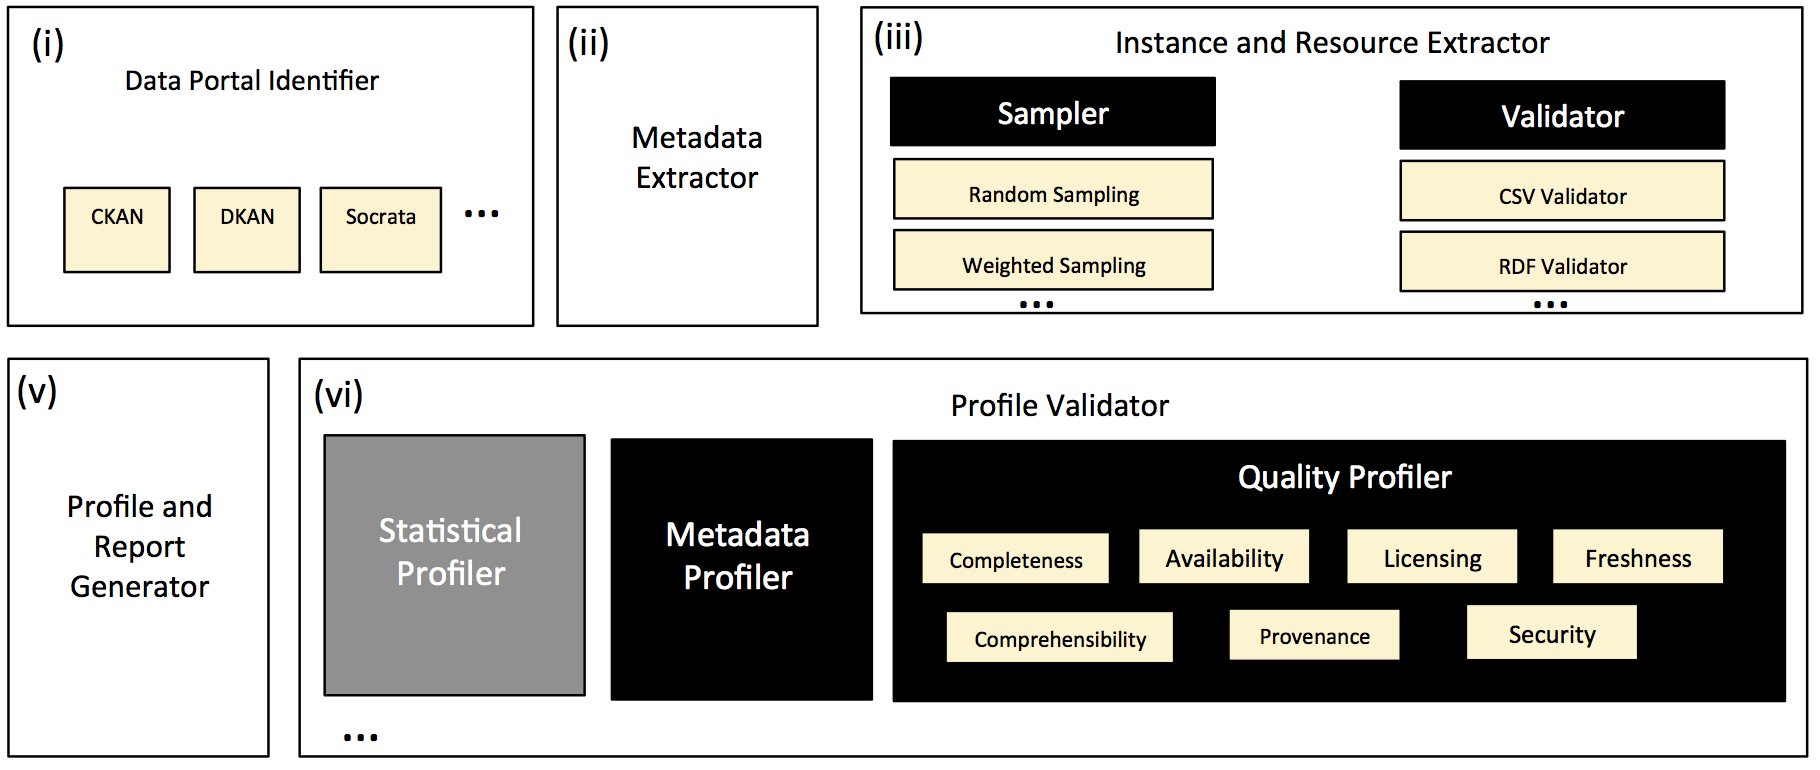
\includegraphics[scale=0.4]{figure-1_architecture.png}
  \caption{Processing pipeline for objective dataset quality assessment}
  \label{fig:1}
\end{figure}

For this paper, we have extended Roomba with a new quality module to measure datasets quality. We have implemented 7 submodules that will check various dataset quality indicators. Various additional quality measures can be easily plugged in/out.\\

Data portals can be considered as data access points providing tools to facilitate data publishing, sharing, searching and visualization. CKAN\footnote{http://ckan.org} is the world's leading open-source data portal platform powering websites and the target of our tool.\\
We have identified that most of the dataset quality issues can be assessed by examining the accompanying dataset metadata. Building a standard metadata model is not the scope of this paper, and since we focus on CKAN-based portals, we assess the quality issues using the CKAN standard model\footnote{http://demo.ckan.org/api/3/action/package\_show?id=adur\_district\_spending}. Table 2 shows the various quality indicators checked by our tool.

\begin{table}[h!]
\begin{center}
{
\small
\begin{tabular}{|c|L|}

\hline
Quality Indicator & Assessment Method\tabularnewline
\hline
\hline
1 & Check if there is a valid metadata file by issuing a \texttt{package\_show} request to the CKAN API\tabularnewline
\hline
2 & Check if the \texttt{format} field for the dataset resources is defined and valid\tabularnewline
\hline
3 & Check the \texttt{resource\_type} field with the following possible values \texttt{file, file.upload, api, visualization, code, documentation}\tabularnewline
\hline
4 & Check the resources \texttt{format} field for \texttt{meta/void} value\tabularnewline
\hline
5 & Check the resources \texttt{size} or the \texttt{triples} extras fields\tabularnewline
\hline
6 & Check the \texttt{format} and \texttt{mimetype} fields for resources\tabularnewline
\hline
7 & Check if the dataset has a \texttt{topic} tag and if it is part of a valid group in CKAN\tabularnewline
\hline
9 & Check if the dataset and all its resources have has a valid URI \tabularnewline
\hline
18 & Check if there is a dereferencable resource with a description containing string \textit{dump}\tabularnewline
\hline
19 & Check if there is a dereferencable resource with \texttt{resource\_type} of type \texttt{api}\tabularnewline
\hline
20 & Check if all the links assigned to the dataset and its resources are dereferencable\tabularnewline
\hline
21 & Check if the dataset contains valid \texttt{license\_id} and \texttt{license\_title}\tabularnewline
\hline
22 & Check if the \texttt{license\_url} is dereferencable\tabularnewline
\hline
24 & Check if the dataset and its resources contain the following metadata fields \texttt{metadata\_created, metadata\_modified, revision\_timestamp, cache\_last\_updated}\tabularnewline
\hline
25 & Check if the \texttt{content-type} extracted from the a valid HTTP request is equal to the corresponding \texttt{mimetype} field.\tabularnewline
\hline
26 & Check if the \texttt{content-length} extracted from the a valid HTTP request is equal to the corresponding \texttt{size} field.\tabularnewline
\hline
28,29 & Check that all the links are valid HTTP scheme URIs\tabularnewline
\hline
37 & Check if there is at least one resource with a \texttt{format} value corresponding to one of \texttt{example/rdf+xml, example/turtle, example/ntriples, example/x-quads, example/rdfa, example/x-trig}\tabularnewline
\hline
39 & Check if the dataset and its tags and resources contain general metadata
\texttt{id, name, type, title, description, URL, display\_name, format}\tabularnewline
\hline
40 & Check if the dataset contain valid \texttt{author\_email} or \texttt{maintainer\_email} fields\tabularnewline
\hline
44 & Check if the dataset and its resources contain provenance metadata \texttt{maintainer, owner\_org, organization, author, maintainer\_email, author\_email}\tabularnewline
\hline
46 & Check if the dataset contain and its resources contain versioning information \texttt{version, revision\_id} \tabularnewline
\hline

\end{tabular}
}
\caption{Objective Quality Assessment Methods for CKAN\-based Data Portals}
\end{center}
\end{table}

In our framework, we have presented 30 objective quality indicators related to dataset and links quality. Roomba quality module is able to assess and score 23 of them. We excluded security related quality indicators as LOD cloud group members should not restrict access to their datasets.

\subsection{Quality Score Calculation}

A CKAN portal contains a set of datasets $\textbf{D} = \{D_1,...D_n\}$. We denote the set of resources $R_i = \{r_1,...,r_k\}$, groups $G_i = \{g_1,...,g_k\}$ and tags $T_i = \{t_1,...,t_k\}$ for $D_i \in \textbf{D} (i=1,...,n)$ by $  \textbf{R}=\{R_1,...,R_n\}, \textbf{G}=\{G_1,...,G_n\}$ and $\textbf{T}=\{T_1,...,t_n\}$ respectively.\\
Our quality framework contains a set of measures $\textbf{M} = \{M_1,...,M_n\}$. We denote the set of quality indicators $Q_i = \{q_1,...,q_k\}$ for $M_i \in \textbf{M} (i=1,...,n)$ by $\textbf{Q} = \{Q_1,...,Q_n\}$. Each quality indicator has a weight, context and a score $Q_i<weight, context, score>$. In Roomba, all the weights are equal and set to 1. However, they can be adjusted manually to rank the quality indicators. Each $Q_i$ of $M_i$ (for $i$ = 1,...$n$) is applied to one or more of the resources, tags or groups. The indicator context is defined where $\exists Q_i \in \textbf{R} \cup \textbf{G} \cup \textbf{T}$.\\
The quality indicator score is based on a ratio between the number of violations $\textbf{V}$ and the total number of instances where the rule applies $\textbf{T}$ multiplied by the specified weight for that indicator.

\begin{equation}
 Q\textrm{ weightedscore} = (V/T) * Q<weight>
\end{equation}

$Q\textrm{ weightedscore}$ is an error ratio. A quality measure score should reflect the alignment of the dataset with respect to the quality indicators. The quality measure score \textbf{M} is calculated by dividing the weighted quality indicator scores sum by the total number of instances in its context, as the following formula shows:

\begin{equation}
 M =  1 - ((\sum_{i=1}^{n} Q\textrm{ weightedscore}) / \mid Q\textrm{ context} \mid )
\end{equation}

\lstset{basicstyle=\small, backgroundcolor=\color{white}, breaklines=false, frame=single, caption={Excerpt of the LOD cloud group quality report}, label=report, captionpos=b}
\begin{lstlisting}
 =================================================================================
                             Dataset Quality Report
 =================================================================================
 completeness quality Score      :   50.22%
 availability quality Score      :   26.22%
 licensing quality Score         :   19.59%
 freshness quality Score         :   79.49%
 correctness quality Score       :   72.06%
 comprehensibility quality Score :   31.62%
 provenance quality Score        :   74.07%
 Average total quality Score     :   50.47%
 =================================================================================
                         Quality Indicators Average Error %
 =================================================================================
 Quality Indicator : Supports multiple serializations: 11.35%
 Quality Indicator : Has different data access points: 19.31%
 Quality Indicator : Uses datasets description vocabularies: 88.80%
 Quality Indicator : Existence of descriptions about its size: 86.30%
 Quality Indicator : Existence of descriptions about its structure: 83.67%
\end{lstlisting}

\section{Experiments and Evaluation}

In this section, we provide the experiments and evaluation of the proposed framework. All the experiments are reproducible by our tool and their results are available on the its Github repository.\\
We have run the framework on the LOD cloud containing 259 datasets at the time of writing this paper. We ran the instance and resource extractor in order to cache the metadata files for these datasets locally and ran the quality assessment process which took around two hours and a half hour on a 2.6 Ghz Intel Core i7 processor with 16GB of DDR3 memory machine.\\

We found out that licensing, availability and comprehensibility had the worst quality measures scores: 19.59\%, 26.22\% and 31.62\% respectively. On the other hand, the LOD cloud datasets have good quality scores for freshness, correctness and provenance as most of the datasets have an average of ~75\% for each one of those measures.

\begin{figure}[ht]
  \centering
    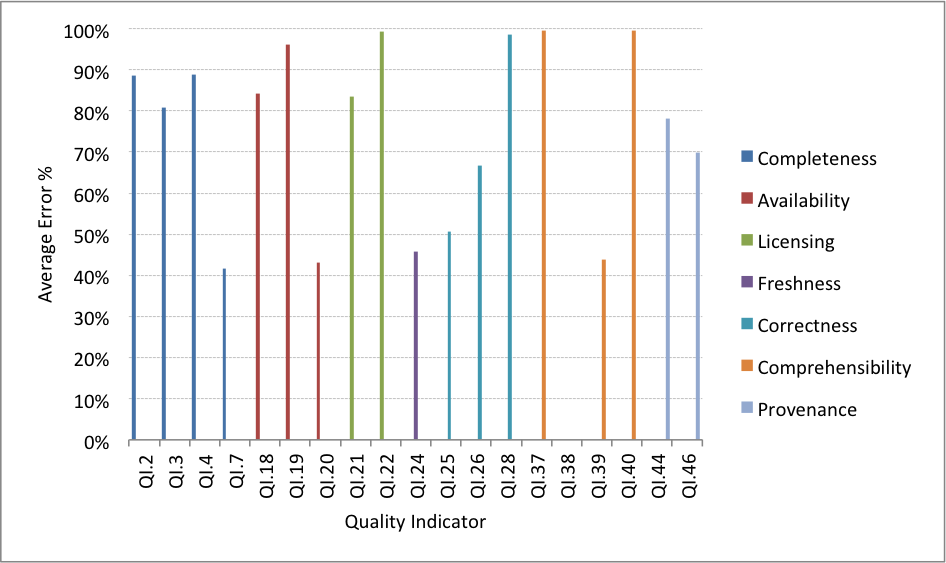
\includegraphics[height=6.5cm, width=12cm]{LOD_quality_indicators_grouped.png}
  \caption{Average quality score per quality indicator for LOD group}
  \label{fig:2}
\end{figure}

Figure \ref{fig:2} shows the average errors percentage in quality indicators grouped by the corresponding measures. After examining the results, we notice that the worst quality indicators scores are for the comprehensibility measure where 99.61\% of the datasets did not have valid exemplary RDF file (QI.37) and did not define valid point of contact (QI.40). Moreover, we noticed that 96.41\% of the datasets queryable endpoints (SPARQL endpoints) failed to respond to direct queries (QI.19). After careful examination, we found that the cause was incorrect assignment for metadata fields. Data publishers specified the resource \texttt{format} field as an \texttt{api} instead of the specifying the \texttt{resource\_type} field.\\

To drill down more on the availability issues, we generated a metadata profile assessment report using Roomba's metadata profiler. We found out that 25\% of the datasets access information (being the dataset URL and any URL defined in its groups) has issues related to them (missing or unreachable URLs).
Three datasets (1.15\%) did not have a URL defined while 45 datasets (17.3\%) defined URLs were not accessible at the time writing this paper. Out of the 1068 defined resources 31.27\% were not reachable. All these issues resulted in a 26.22\% average availability score. This can highly affect the usability of those datasets especially in an enterprise context.

\section{Linked Data Quality Tools}
In this section, we present the results of our survey on the Linked Data quality tools. There exists a number of data quality frameworks and tools that are either standalone or implemented as modules in data integration tools. These approaches can be classified into automatic, semi-automatic, manual or crowd sourced approaches.

\subsection{Information Quality}

RDF is the standard to model information in the Semantic Web. Linked Data publishers can pick from a plethora of tools that can automatically check their RDF files for quality problems\footnote{http://www.w3.org/2001/sw/wiki/SWValidators}. Syntactic RDF checkers are able to detect errors in RDF documents like the W3C RDF Validator\footnote{http://www.w3.org/RDF/Validator/}, RDF:about validator and Converter\footnote{http://rdfabout.com/demo/validator/} and The Validating RDF Parser (VRP)\footnote{http://139.91.183.30:9090/RDF/VRP/index.html}. The RDF Triple-Checker\footnote{http://graphite.ecs.soton.ac.uk/checker/} is an online tool that helps find typos and common errors in RDF data. Vapour\footnote{http://validator.linkeddata.org/vapour} \cite{Berrueta08cookinghttp} is a validation service to check whether semantic Web data is correctly published according to the current best practices \cite{tim:linkedata}.\\
ProLOD \cite{Bohm2010}, ProLOD++ \cite{6816740}, Aether \cite{makela-aether-2014} and LODStats \cite{demter-2012-ekaw} are not purely quality assessment tools. They are Linked Data profiling tools providing clustering and labeling capabilities, schema discovery and statistics about data types and patterns. The statistics are about properties distribution, link-to-literal ratio, number of entities and RDF triples, average properties per entity and average error.

\subsection{Modeling Quality}

Reusing existing ontologies is a common practice that Linked Data publishers are always trying to adopt. However, ontologies and vocabularies development is often a long error-prone process especially when many contributors are working consecutively or collaboratively \cite{Suominen2013}. This can introduce deficiencies such as redundant concepts or conflicting relationships \cite{harpring_introduction_2010}. Getting to choose the right ontology or vocabulary is vital to ensure modeling correctness and consistency.\\

\subsubsection{Semi-automatic Approaches}

DL-Learner \cite{Lehmann_dl-learner:learning} uses supervised machine learning techniques to learn concepts from user-provided examples. CROCUS \cite{wasabi_crocus} applies a cluster-based approach for instance-level error detection. It validates identified errors by non-expert users and iterate to reach higher quality ontologies that can be safely used in industrial environments.

\subsubsection{Automatic Approaches}

qSKOS\footnote{https://github.com/cmader/qSKOS} \cite{Mader2012} scans SKOS vocabularies to provide reports on vocabulary resources and relations that are problematic. PoolParty checker\footnote{http://www.poolparty.biz/} is an online service based on qSKOS. Skosify \cite{Suominen:2012:IQS:2413941.2413985} supports OWL and RDFS ontologies by converting them into well-structured SKOS vocabularies. It includes automatic correction abilities for quality issues that have been observed by reviewing vocabularies on the Web. The OOPS! pitfall scanner \cite{oops} evaluates OWL ontologies against a rules catalog and provides the user with a set of guidelines to solve them. ASKOSI\footnote{http://www.w3.org/2001/sw/wiki/ASKOSI} retrieves vocabularies from different sources, stores and displays the usage frequency of the different concepts used by different applications. It promotes reusing existing information systems by providing better management and presentation tools.\\ Some errors in RDF will only appear after reasoning (incorrect inferences). In \cite{conf/owled/SirinSW08}\cite{conf/hicss/TaoDM09} the authors perform quality checking on OWL ontologies using integrity constraints involving the Unique Name Assumption (UNA) and the Closed World Assumption (CWA). Pellet\footnote{http://clarkparsia.com/pellet} provides reasoning services for OWL ontologies. It incorporates a number of heuristics to detect and repair quality issues among disjoint properties, negative property assertions and reflexive, irreflexive, symmetric, and anti-symmetric properties. Eyeball\footnote{http://jena.sourceforge.net/Eyeball/} provides quality inspection for RDF models (including OWL). It provides checks for a variety of problems including the usage of unknown predicates, classes, poorly formed namespaces, literal syntax validation, type consistency and other heuristics. RDF:Alerts\footnote{http://swse.deri.org/RDFAlerts/} provides validation for many issues highlighted in \cite{Hogan2010} like misplaced, undefined or deprecated classes or properties.\\


\subsection{Dataset Quality}
Considering the large amount of available datasets in the Linked Open Data, users have a hard time trying to identify appropriate datasets that suit certain tasks. The most adopted approaches are based on link assessment. Provenance-based approaches and entity-based approaches are also used to compute not only dataset rankings, but also rankings on the entity level.\\

\subsubsection{Manual Ranking Approaches}

Sieve \cite{Mendes2012} is a framework for expressing quality assessment and fusion methods. It is implemented as a component of the Linked Data Integration Framework (LDIF)\footnote{http://ldif.wbsg.de/}. Sieve leverages the LDIF provenance metadata as quality indicators to produce quality assessment scores. However, despite its nice features, it is only targeted to perform data fusion based on user-configurable conflict resolution tasks. Moreover, since Sieve main input is provenance metadata, it is only limited to domains that can provide such metadata associated with their data.

SWIQA \cite{Furber2011a} is a framework providing policies or formulas controlling information quality assessment. It is composed of three layers: data acquisition, query and ontology layers. It uses query templates based on the SPARQL Inferencing Notation (SPIN)\footnote{http://spinrdf.org/} to express quality requirements. The queries are built to compute weighted and unweighted quality scores. At the end of the assessment, it uses vocabulary elements to annotate important values of properties and classes, assigning inferred quality scores to ontology elements and classifying the identified data quality problems.

\subsubsection{Crowd-sourcing Approaches}

There are several quality issues that can be difficult to spot and fix automatically. In \cite{Acosta2013} the authors highlight the fact that the RDFification process of some data can be more challenging than others, leading to errors in the Linked Data provisioning process that needs manual intervention. This can be more visible in datasets that have been semi-automatically translated to RDF from their primary source (the best example for this case is DBpedia \cite{bizer_dbpedia_2009}). The authors introduce a methodology to adjust crowdsourcing input from two types of audience: 1) Linked Data experts, researchers and enthusiasts through a contest to find and classify erroneous RDF triples and 2) Crowd-sourcing through the Amazon Mechanical Turk\footnote{https://www.mturk.com/}.

TripleCheckMate \cite{Kontokostas2013} is a crowd-sourcing tool used by the authors to run out their assessment supported by a semi-automatic quality verification metrics. The tool allows users to select resources, identify and classify possible issues according to a pre-defined taxonomy of quality problems. It measures inter-rater agreements, meaning that the resources defined are checked multiple times. These features turn out to be extremely useful to analyze the performance of users and allow better identification of potential quality problems. TripleCheckMate is used to identify accuracy issues in the object extraction (completeness of the extraction value for object values and data types), relevancy of the extracted information, representational consistency and interlinking with other datasets.

\subsubsection{Semi-automatic Approaches}

Luzzu \cite{DBLP:journals/corr/DebattistaLLA14} is a generic Linked Data quality assessment framework. It can be easily extended through a declarative interface to integrate domain specific quality measures. The framework consists of three stages closely corresponding to the methodology in \cite{DBLP:conf/i-semantics/RulaZ14}. They believe that data quality cannot be tackled in isolation. As a result, they require domain experts to identify quality assessment metrics in a schema layer. Luzzu is ontology driven. The core vocabulary for the schema layer is the Dataset Quality Ontology (daQ) \cite{DBLP:conf/www/Debattista0A14}. Any additional quality metrics added to the framework should extend it.

RDFUnit\footnote{http://github.com/AKSW/RDFUnit} is a tool centered around the definition of data quality integrity constraints \cite{Kontokostas:2014:TEL:2566486.2568002}. The input is a defined set of test cases (which can be generated manually or automatically) presented in SPRAQL query templates. One of the main advantages for this approach is the ability to discover quality problems beyond conventional quality heuristics by encoding domain specific semantics in the test cases.

LiQuate \cite{conf/otm/RuckhausBV13} is based on probabilistic models to analyze the quality of data and links. It consists of two main components: A Bayesian Network builder and an ambiguity detector. They rely on data experts to represent probabilistic rules. LiQuate identifies redundancies (redundant label names for a given resource), incompleteness (incomplete links among a given set of resources) and inconsistencies (inconsistent links).

Quality Assessment of Data Sources (Flemming's Data Quality Assessment Tool)\footnote{http://linkeddata.informatik.hu-berlin.de/LDSrcAss/datenquelle.php} calculates data quality scores based on manual user input. The user should assign weights to the predefined quality metrics and answer a series of questions regarding the dataset. These include, for example, the use of obsolete classes and properties by defining the number of described entities that are assigned disjoint classes, the usage of stable URIs and whether the publisher provides a mailing list for the dataset. The main disadvantage for using this tool is the manual intervention which requires deep knowledge in the dataset examined. Moreover, the tool lacks support for several quality concerns like completeness or consistency.

LODGRefine \cite{conf/i-semantics/Verlic12} is the Open Refine\footnote{http://openrefine.org/} of Linked Data. It does not act as a quality assessment tool, but it is powerful in cleaning and refining raw instance data. LODGRefine can help detect duplicates, empty values, spot inconsistencies, extract Named Entities, discover patterns and more. LODGRefine helps in improving the quality of the dataset by improving the quality of the data at the instance level.\\

\subsubsection{Automatic Ranking Approaches}

The Project Open Data Dashboard\footnote{http://labs.data.gov/dashboard/} tracks and measures how US government websites implement the Open Data principles to understand the progress and current status of their public data listings. A validator analyzes machine readable files e.g. JSON files for automated metrics like the resolved URLs, HTTP status and content-type. However, deep schema information about the metadata is missing like description, license information or tags. \\
Similarly on the LOD cloud, the Data Hub LOD Validator\footnote{http://validator.lod-cloud.net/} gives an overview of Linked Data sources cataloged on the Data Hub. It offers a step-by-step validator guidance to check a dataset completeness level for inclusion in the LOD cloud. The results are divided into four different compliance levels from basic to reviewed and included in the LOD cloud. Although it is an excellent tool to monitor LOD compliance, it still lacks the ability to give detailed insights about the completeness of the metadata and overview on the state of the whole LOD cloud group and is very specific to the LOD cloud group rules and regulations.\\

\indent \\{\bf Link-based Approaches}

The basic idea behind link assessment tools is to provide rankings for datasets based on the cardinality and types of the relationships with other datasets. Traditional link analysis has proven to be an effective way to measure the quality of Web documents search. Algorithms like PageRank \cite{Lawrence981} and HITS \cite{Kleinberg:1999} became successful based on the assumption that a certain Web document is considered to have higher importance or rank if it has more incoming links that other Web documents \cite{Brin:1998}\cite{Chakrabarti99miningthe}.\\ However, the basic assumption that links are equivalent does not suit the heterogeneous nature of links in the Linked Open Data. Thus, the previous approaches fall short to provide reliable rankings as the types of the links can have a direct impact on the ranking computation \cite{Toupikov2009}.\\ The first adaption of PageRank for Semantic Web resources was the Ontology Rank algorithm implemented in the Swoogle search engine \cite{Ding2004}. They use a rational random surfing model that takes into account the different types of links between discovered sets and compute rankings based on three levels of granularity: documents, terms and RDF graphs. ReConRank \cite{Hogan06reconrank:a} rankings are computed at query time based on two levels of granularity: resources and context graphs. DING \cite{Toupikov2009} adapted the PageRank to rank datasets based on their interconnections. DING can also automatically assign weights to different link types based on the nature of the predicate involved in the link.\\Broken links are a major threat to Linked Data. They occur when resources are removed, moved or updated. DSNotify\footnote{http://www.cibiv.at/~niko/dsnotify/}\cite{cs142} is a framework that informs data consumers about the various types of events that occur on data sources. Their approach is based on an indexing infrastructure that extracts feature vectors and stores them to an index. A monitoring module detects events on sources and write them to a central event log which pushes notifications to registered applications.\\ LinkQA \cite{Gueret2012} is a fully automated approach which takes a set of RDF triples as an input and analyses it to extract topological measures (links quality). However, the authors depend only on five metrics to determine the quality of data (degree, clustering coefficient, centrality, sameAs chains and descriptive richness through sameAs).\\

\noindent{\bf Provenance-based Approaches}

Provenance-based assessment methods are an important step towards transparency of data quality in the Semantic Web. In \cite{Hartig09usingweb}\footnote{http://trdf.sourceforge.net} the authors use a provenance model as an assessment method to evaluate the timeliness of Web data. Their model identifies types of ``provenance elements'' and the relationships between them. Provenance elements are classified into three types: actors, executions and artifacts. The assessment procedure is divided into three steps: 1) Creating provenance graph based on the defined model 2) Annotating the graph with impact values 3) Calculating the information quality score. In \cite{Flouris2012} the authors describe a set of provenance-based assessment metrics to support quality assessment and repair in Linked Open Data. They rely on both data and metadata and use indicators like the source reputation, freshness and plausibility. In \cite{Harth2009} the authors introduce the notion of naming authority which connects an identifier with the source to establish a connection to its provenance. They construct a naming authority graph that acts as input to derive PageRank scores for the data sources.\\

\noindent{\bf Entity-based Approaches}

Sindice \cite{Delbru2010} uses a set of techniques to rank Web data. They use a combination of query dependent and query independent rankings implemented in the Semantic Information Retrieval Engine (SIREn)\footnote{http://siren.sindice.com/} to produce a final entity rank. Their query dependent approach rates individual entities by aggregating the the score of the matching terms with a term frequency - inverse subject frequency (tf-isf) algorithm. Their query independent ranking is done using hierarchical links analysis algorithms \cite{Delbru2010a}. The combination of these two approaches is used to generate a global weighted rank based on the dataset, entities and links ranks.\\

\subsection{Queryable End-point Quality}

The availability of Linked Data is highly dependent on the performance qualities of its queryable end-points. The standard query language for Semantic Web resources is SPARQL. As a result, we focus on tools measuring the quality of SPARQL endpoints. In \cite{Buil-Aranda2013}\footnote{http://labs.mondeca.com/sparqlEndpointsStatus/} the authors present their findings to measure the discoverability of SPARQL endpoints by analyzing how they are located and the metadata used to describe them. In addition to that, they also analyze endpoints interoperability by identifying features of SPARQL 1.0 and SPARQL 1.1 that are supported. The authors tackled the endpoints efficiency by testing the time taken to answer generic, content-agnostic SPARQL queries over HTTP.\\

\noindent

\textbf{Summary}
\indent \\\\
\indent We notice that there is a plethora of tools (syntactic checkers or statistical profilers) that automatically check the quality of information at the entities level. Moreover, various tools can automatically check the models against the objective quality indicators mentioned. OOPS! covers all of them with additional support for the other common modeling pitfalls in \cite{DBLP:conf/ic3k/KeetSP13}. PoolParty covers also a wide set of those indicators but it targets SKOS vocabularies only. However, we notice a lack in automatic tools to check the dataset quality especially in its completeness, licensing and provenance measures. Table 3 summarizes the automatic dataset quality approaches that have implemented tools (full circle denotes full quality indicator assessment, while half circle denoted partial assessment). As can be seen in this table Roomba covers most of the quality indicators with its focus on completeness, correctness provenance and licensing. Roomba is not able to check the existence of information about the kind and number of used vocabularies (QI.8), license permissions, copyrights and attributes (QI.23), exemplary SPARQL query (QI.38), usage of provenance vocabulary (QI.45) and is not able to check the dataset for syntactic errors (QI.27).\\These shortcomings are mainly due to the limitations in the CKAN dataset model. However, syntactic checkers and additional modules to examine vocabularies usage could be easily integrated in Roomba to fix QI.27, QI.8 and QI.45. Roomba's metadata quality profiler can fix QI.23 as we have manually created a mapping file standardizing the set of possible license names and their information\footnote{https://github.com/ahmadassaf/opendata-checker/blob/master/util/licenseMappings.json}. We have also used the open source and knowledge license information\footnote{https://github.com/okfn/licenses} to normalize license information and add extra metadata like the domain, maintainer and open data conformance.

\begin{table}[htp]
\centering
\footnotesize\setlength{\tabcolsep}{2.5pt}
\begin{tabular}{|c|c|c|c|c|c|c|c|c|c|c|c|c|c|c|c|c|c|c|c|c|c|c|c|c|c|c|c|c|c|c|}

\hline
Tool\textbackslash{}Indicator & 1 & 2 & 3 & 4 & 5 & 6 & 7 & 8 & 9 & 18 & 19 & 20 & 21 & 22 & 23 & 24 & 25 & 26 & 27 & 28 & 29 & 37 & 38 & 39 & 40 & 44 & 45 & 46 & 63 & 64\tabularnewline
\hline

\hline
LOV & \ding{108} &  & \ding{108} & \ding{108} & \ding{119} &  & \ding{119} &  & \ding{108} & \ding{108} &  & \ding{108} & \ding{119} &  &  &  &  &  &  &  &  & \ding{108} &  & \ding{119} &  & \ding{108} &  & \ding{108} &  & \tabularnewline

\hline
Data.gov & \ding{108} &  &  &  & \ding{119} & \ding{108} &  &  & \ding{108} &  &  & \ding{108} &  &  &  & \ding{119} & \ding{108} &  &  &  &  &  &  & \ding{108} &  & \ding{119} &  &  &  & \tabularnewline

\hline

Roomba & \ding{108} & \ding{108} & \ding{108} & \ding{108} & \ding{108} & \ding{108} & \ding{108} &  & \ding{108} & \ding{108} & \ding{108} & \ding{108} & \ding{108} & \ding{108} &  & \ding{108} & \ding{108} & \ding{108} & \ding{108} & \ding{108} &  & \ding{108} &  & \ding{108} & \ding{108} & \ding{108} &  & \ding{108} &  & \tabularnewline

\hline
\end{tabular}
\caption{Functional Comparison of Automatic Linked Data quality Tools}
\end{table}

\section{Conclusions and Future Work}

In this paper, we have presented a comprehensive objective quality framework applied to the Linked Open Data. We have built upon our previous work to focus on objective data quality measures. We have identified a total of 64 quality indicators that were mapped when suitable to four main categories (entity, dataset, links, models). We have also surveyed more than 30 different tools that measure different quality aspects of Linked Open Data. We identified several gaps in the current tools and identified the need for a comprehensive evaluation and assessment framework and specifically for measuring quality on the dataset level. As a result, we presented an extension of Roomba (An extensible tool to assess and generate dataset profiles) that covers 82\% of the suggested datasets objective quality indicators.\\
Based on our experiments running Roomba on the LOD cloud, we discovered that the general state of the datasets needs attention as most of them have low completeness, provenance, licensing and comprehensibility quality scores.\\
In future work, we plan to integrate tools assessing models quality in addition to syntactic checkers with Roomba. This will provide a complete coverage of the proposed quality indicators. We also intend to suggest ranked quality indicators to improve the quality report. We also plan to run this tool on various CKAN based data portals and schedule periodic reports to monitor their quality evolution. Finally, at some stage, we plan to extend this tool for other data portal types like DKAN and Socrata.

\bibliographystyle{abbrv}
\bibliography{DQ}

\end{document}


